\section{Introduction}

\subsection{Motivation and Objective}

Virtual Reality technology to immerse in a computer generated scenario simulating a realistic experience because of a created environment similar to the real world is continuously improving and potential users become more and more attracted by the possibilities offered through virtual reality.

Current technology enables the user to look around the artificial world, move in it, and interact with virtual features or items. Therefore continuous development of virtual reality items and features is necessary to improve their functionality as well as expand their possibilities of application. Because of that, our objective is to adjust the actual Cyber Glove and design new use cases to offer the user a better experience and expand the application possibilities of the Cyber Glove in the virtual reality.

Fulfilling this objective, we defined our project plan and our strategy and divided the main aspects into three sub aspects. Therefore all team members were able to specialize better in their chosen sub aspects and progress was guaranteed. The three aspects were defined as followed:


\begin{description}
	\item[Hardware development:] Designing a new Cyber Glove with a new board and its housing as well as implementing three additional bending sensors and a joystick. Renewing the tracking system and changing the battery to improve functionality of the glove and make it lighter and more comfortable to use.
	
	\item[Software development:] Revising and redesigning of the WLAN transmission protocol as well as modifying, customizing and implementing more features by adapting the Arduino code to transmit the sensor values and enable the usage of the Cyber Glove and its new functions in the cave. 
	
	\item[Development and design of new use cases:] Our renewals and development of software and hardware were tested by development and implementation of new use cases. Those use cases simplify it for users to understand the functionality of the Cyber Glove and a new design was implemented to make it easier to immerse in the virtual world using the Cyber Glove in the cave.
\end{description}

Thus, definition of individual goals in the main aspects represent the overall task. The implementation of the overall task improves immersion in the virtual world with the Cyber Glove. Furthermore, structuring of the three main aspects helps to simplify the management and organization within the team.



\subsection{Team and Project Plan}

Interdisciplinary skills should ensure optimal development of the Cyber Glove. Therefore our team consists of 7 members of different disciplines who did contribute their individual knowledge to the project. We divided the group of three Computer Scientists, two Civil Engineers and two Industrial Engineers into smaller project groups. Thereby each group was resolving another challenge of the objectives set.

We have formed the following groups in order to divide the tasks:

\begin{description}
	\item[Hardware team:] Frieder, Fabian
	\item[Software team:] Johanna, Lukas
	\item[Use case team:] Ran, Shant, Johanna, Lukas
	\item[Coordination and management:] Tanja
\end{description}

\begin{figure}
	\centering
	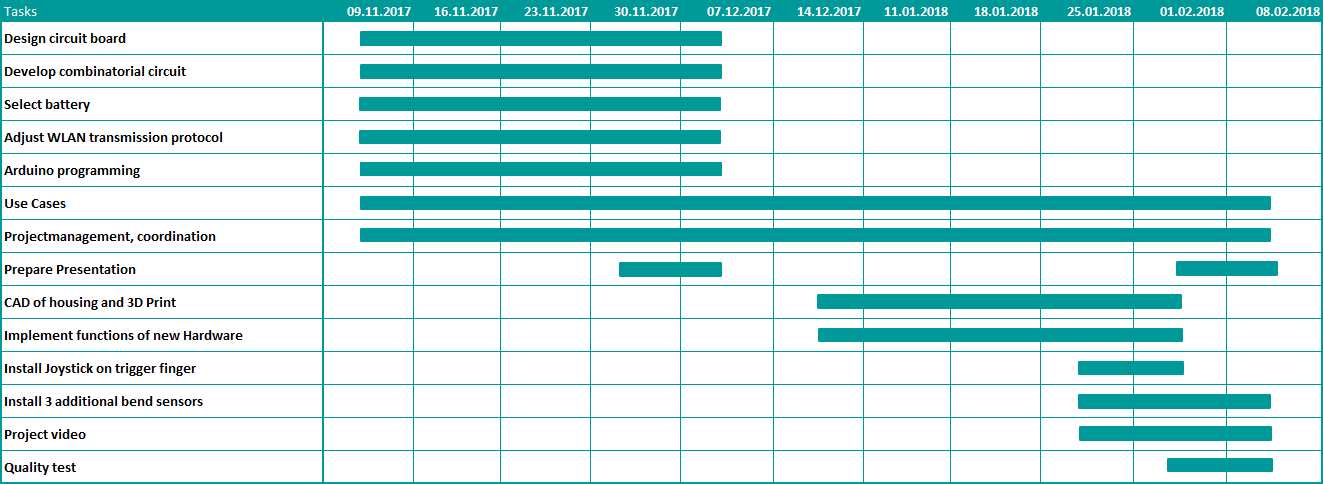
\includegraphics[width=\textwidth]{./images/gantt.png}
	\caption{Gantt chart describing our tasks}
	\label{img:gantt}
\end{figure}

The Gantt chart in Figure \ref{img:gantt} shows the main tasks, together with the scheduled time to fulfill each task.  

First of all we analyzed the current Cyber Glove and discussed challenges and difficulties of further development. It was important to get an insight in the technical state of the Cyber Glove and further explanation regarding hardware and software from our project coordinator. After getting a complete overview we defined the objectives as well as the tasks and divided our team in expert groups. Afterwards we scheduled the tasks and estimated the time necessary to fulfill each task.

In the second phase the hardware group designed the circuit board, developed the combinatorial circuit and selected a battery. Our software group adjusted the WLAN transmission protocol and started Arduino programming. The user case team started to focus on understanding Poly VR software to afterwards start programming new use cases for the Cyber Glove. 

Weekly team meetings were coordinated and held to keep all team members up to date on current progress of the other expert groups. Furthermore those team meetings were a possibility for each sub group to get input and ideas by other sub groups so even though there were existing expert groups, development was still discussed and supported through the whole team. The fact of having team members of very different specializations made the input across groups very profitable and versatile. The second phase closed with the midterm presentations where we presented the current state and developments of the project.

Hereafter the third phase started in which our software team joined the use case group to generate use cases meanwhile they kept on working on the software. The hardware team was responsible to set up the CAD of housing and transmit it to project coordinator for 3D printing. Furthermore the started implementing functions of new hardware. To the same time the new Cyber Glove was designed and to afterwards install joystick and 3 additional bend sensors. All together was connected through soldering of the wires.

The task “prepare presentation” was fulfilled two times, each one week before the mid and final presentation by all team members. Management, coordination and communication, designing the new Cyber Glove by sewing and wiring as well as the project video were the tasks of the project coordinator.

A more detailed description of the individual tasks as well as the identification of problems during the process and the learning effect are discussed below.



